% status: FINAL 2024-2025
% v20240829

\documentclass[12pt,a4paper,english]{article}

%--- Styling preamble ---

%% Essential

\usepackage[T1]{fontenc} % essential for hyphenation and copy/pasting in the final pdf
\usepackage{babel} % english-language support and hy-phen-a-tion. supports many languages. best practice is to set the language as an option to the \documentclass
\usepackage{graphicx} % enhanced support for graphics
\usepackage{amsmath} % essential additional math options
\usepackage{xcolor} % for more color options, and colored text
\usepackage{subcaption}
\usepackage{longtable}

% importing other assignments
\usepackage{pdfpages}

\usepackage[style=ieee]{biblatex}
\addbibresource{references.bib}

%% Recommended packages

\usepackage[margin=2.5cm]{geometry} % to set page margins
\usepackage{comment} % To enable comment blocks that are not interpreted
\usepackage{newtxtext,newtxmath} % changes fonts for better on-screen reading


%% Essential in Physics Lab: Skills

\usepackage{siunitx} % for appropriate value + unit + error formatting
    \sisetup{separate-uncertainty} % write error out with ±
\usepackage{titling} % for title page with abstract
\usepackage[nottoc]{tocbibind} % bibliography in ToC

\usepackage[hyperindex,colorlinks,linktoc=all]{hyperref} % for clickable links in pdf. essential feature for the TAs! should often be the last package (with the exceptions below)
\usepackage{caption} % to point hyperref links to top of figure/table. put after hyperref
\usepackage{bookmark} % to improve hyperref pdf bookmarks. put after hyperref
\usepackage[nameinlink]{cleveref} % Better linking, e.g. to multiple figures and tables. Goes after hyperref
    \urlstyle{same}
    \hypersetup{ % hyperref/bookmark/cleveref package setup parameters
            colorlinks=true,
            linkcolor=purple,
            filecolor=teal,
            urlcolor=olive,
            citecolor=teal,
            bookmarksopen=true,
            bookmarksopenlevel=0,
            pdflang=en,
            pdfpagemode=UseOutlines,
            pdfstartview=FitB,
            pdfpagelayout=OneColumn,
            pdftitle={Experiment X Report},
            pdfauthor={M. Doe, P.P. Recies},
        }

% Stuff for code & algorithms
\usepackage{listings}

\usepackage[utf8]{inputenc}
\usepackage[T1]{fontenc}
\usepackage{listings}
\usepackage{xcolor}
 
\definecolor{codegreen}{rgb}{0,0.6,0}
\definecolor{codegray}{rgb}{0.5,0.5,0.5}
\definecolor{codepurple}{rgb}{0.58,0,0.82}
\definecolor{backcolour}{rgb}{0.95,0.95,0.92}
 
\lstdefinestyle{python}{
    backgroundcolor=\color{backcolour},   
    commentstyle=\color{codegreen},
    keywordstyle=\color{magenta},
    numberstyle=\tiny\color{codegray},
    stringstyle=\color{codepurple},
    basicstyle=\footnotesize,
    breakatwhitespace=false,         
    breaklines=true,                 
    captionpos=b,                    
    keepspaces=true,                 
    numbers=left,                    
    numbersep=5pt,                  
    showspaces=false,                
    showstringspaces=false,
    showtabs=false,                  
    tabsize=2
}
\lstset{style=python}

\usepackage{algorithm}

%% Packages not in this example, but that you might want to use:


% General

\usepackage{enumitem} % improve enumeration lists
\usepackage{isodate} % for date formatting
\usepackage{nameref} % to refer to section names themselves, not the number


% Figure options

\usepackage{subcaption} % sub-captions. put after package "caption"
\usepackage{wrapfig}
\usepackage{float}


% Math

\usepackage{bm} % for bold face in math environment (recommended by AMS style guide)
\usepackage{mathtools} % for definition symbol :=

% Options for Hyperref and related packages that were used in 2024 in the manuals

\urlstyle{same}
\hypersetup{ % bookmark/hyperref package setup parameters
        colorlinks=true,
        linkcolor=purple,
        filecolor=teal,
        urlcolor=olive,
        citecolor=teal,
        bookmarksopen=true,
        bookmarksopenlevel=0,
        pdflang=en,
        pdfpagemode=UseOutlines,
        pdfstartview=FitB,
        pdfpagelayout=OneColumn,
    }
\hypersetup{ % PDF metadata
    pdftitle={NLP Assignment 3},
    pdfauthor={Teun Boersma and Marcus Persson},
    }


%--- End of styling preamble ---


% General info for title page
\title{
    \vspace*{-2cm}
    \includegraphics[width=\textwidth]{./img/rugr_fse_logoen_rood_cmyk.eps} \\[1.5cm]
   \\ % insert title here
    {\Large Natural Language Processing \\ }
    {\large{Assignment 3}}
}
\author{Teun Boersma (S5195179),\\ Marcus Persson (S5343798),\\ Julian Sprietsma (S5096219)}
\date{\today}


% Let's go!
\begin{document}

% Title page
\begin{titlingpage}   
    \maketitle
\end{titlingpage}


% Table of Contents (ToC)
{   
    \thispagestyle{empty} % no page number for ToC
    \hypersetup{linkcolor=black} % black links for ToC aesthetics
    \tableofcontents
    \clearpage
}

\section{Dataset \& Setup}
The main focus of this project is to compare the performance of three models. As a baseline model, we are using a Support Vector Machine (SVM), this has been developed in Assignment 1. We will give a succinct summary of the results here. For a full assessment, the full report of Assignment 1 has been included in Appendix \ref{ap:ass1}. Similarly, we will be comparing to a more complex neural model, for this we will be using a Bidirectional Long Short Term Memory model, the results and model architecture will be summarised here; a full assessment can be found in the Assignment 2 report in Appendix \ref{ap:ass2}. This report details the finetuning procedure for the largest model based on a distilled uncased version of DistilBERT \cite{sanh2020distilbertdistilledversionbert}.

This project focuses on the AGNews Dataset, created by Zhang et al. \cite{AGNews}. The dataset consists of 120k training datapoints and 7.6k testing points. Each datapoint consists of a title and a description of a news article. These are around 45 and 200 characters long on average. Each article is categorised based on topic. The set of labels consists of World, Sports, Business and Sci/Tech ($C=4$, $y\in\{1,2,3,4\}$). This project aims to investigate the performance of baseline models on this task. For hyperparameter tuning and testing, a random development split of 10\% was taken from the training set.

For the purpose of word embedding, a different method was used for each model. For the baseline model, a Term Frequency Inverse Document Frequency (TF-IDF) Vectorizer as implemented in Scikit-Learn \cite{scikit-learn} was fitted on the training set and used. The BiLSTM uses a Word2Vec model. 

The DistilBERT Transformer uses a tokeniser based on the WordPiece algorithm. Specifically, the transformer encodes the news article text into input identifiers and attention masks.  Truncation and padding to a maximum length of 256 tokens is applied to ensure uniform input dimensions. The model receives input tensors where the input IDs and attention masks are stacked along the final dimension, then being processed into a one-hoted encoded format to represent the four classes.

\section{Models}
\subsection{Baseline Results}
\subsubsection{Support Vector Machine}
An SVM attempts to fit an optimal separating hyperplane between each pair of classes. Since this cannot be done perfectly, it is necessary to define some slack on the loss, the extent to which this is done is parameterised by the parameter $C$.
The SVM was chosen to use $C=10^{-1}$, based on a grid search. Following this, the SVM reported, for the development set, an accuracy of 0.8776
and a weighted F1-score of 0.8769; for the test set, the model reported an accuracy of 0.7661. 

\subsubsection{Long Short-Term Memory}
The LSTM is a gated Recurrent Neural Network. It possesses, aside from the hidden state vector $\boldsymbol{h}_t$, also a cell state $\boldsymbol{c}_t$. This cell state allows the model to better capture long-range dependencies. Which information is stored/kept/used is controlled through element-wise multiplication with learned gates. 

As for the present task, the full data is known in advance, a bidirectional variant is used, which runs both forward and backwards across the document. 

After evaluating the model reported, for the development set, an accuracy of 0.8992 and a weighted
F1-score of 0.8990; for the test set, the model reported an accuracy of 0.9268 and a weighted
F1-score of 0.9268. An ablation study was also conducted, where it was concluded that the model performs when trained on longer sequences. With a strong resilience due to preprocessing decisions where the title of each article is placed at the start of each document. 

\subsection{DistilBERT}
\subsubsection{Architecture \& Pre-Training}
% Transformer Encoder architecture
The BERT family of models is based on the transformer architecture. A diagram of this architecture can be seen in Figure \ref{fig:diagram}. The first step is the input embeddings; here, the tokeniser tokenises the input document and creates a vector representation for each. These representations are tracked through unique IDs. Next, positional encoding, based on the orthogonality of sinusoids, is used to add a representation of the position in the document, which is kept throughout the following layers. The multi-head attention consists of multiple self-attention modules which each focus on different parts of the input. The fact that each attention head outputs a linear combination of the input embeddings highlights the need for positional encoding. The next layer is a feedforward network, which deals with completing the task. After each layer, the input is added to the layer's output through residual connections (which helps in gradient propagation), and the total is normalised to zero mean unit standard deviation. The DistilBert model we used is a smaller (Distilled) version of the standard BERT model; it consists of six of these previously explained transformer layers, totalling 67M parameters \cite{sanh2020distilbertdistilledversionbert}.

For our project, we used a pretrained version of this model, which was subsequently fine-tuned on the news topic classification task. The pretraining tasks for BERT are masked language modelling, where randomly masked tokens need to be predicted, as well as next sentence prediction, where two sentences are given, and the model is tasked with predicting whether these are two consecutive sentences or not. In the knowledge distillation process, a smaller student model (DistilBERT) is tasked with replicating the behaviour of the teacher model (BERT). DistilBERT retains most of the performance of BERT while being a lot easier to run, which is why we opted for this model \cite{sanh2020distilbertdistilledversionbert}.

\begin{figure}[h]
    \centering
    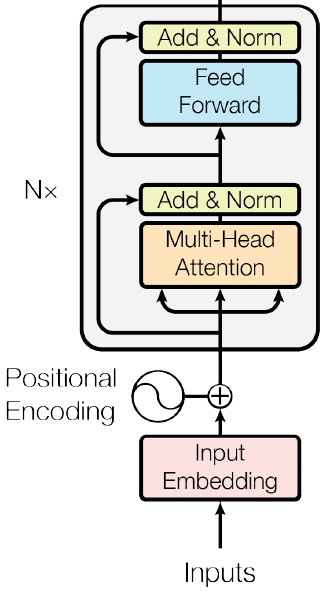
\includegraphics[height=0.3\textheight]{reports//assignment3//img/diagram.png}
    \caption{Diagram of the Encoder Transformer Architecture (taken from \textcite{castellucci2019transformerdiagram})}
    \label{fig:diagram}
\end{figure}

\subsubsection{Fine-Tuning Procedure}
The model was fine-tuned on the AGNews Topic classification dataset using a maximum of 20 epochs. Early stopping was used with a patience of 3 epochs without improvement. When early stopping is triggered, the model gets reverted to the state with the lowest validation loss. The fine-tuning used the AdamW optimiser as implemented in PyTorch \cite{paszke2019pytorchimperativestylehighperformance}. A learning rate of $2\times10^{-5}$ was used. 

\section{Experimental Protocol}
Details on the exact training conditions of the baseline models can be found in Appendix \ref{ap:ass1} and \ref{ap:ass2}. The models are compared on the following metrics: Accuracy, F1-score and a Confusion Matrix. Additionally, a qualitative error analysis is carried out where the differences in mistakes to the baseline models are emphasised. Additionally, a robustness evaluation is carried out. This is used to evaluate how the model performs in certain conditions. Two methods were used, firstly, an evaluation was carried out on the testing data of a certain sequence length, sorted into bins with documents of 0-50, 50-100, 100-150, 150-200, 200-250 and 250-300 tokens. Secondly, the model was evaluated on data with 10 keywords removed for each class to see how reliant the model is on specific class-related words appearing in the samples.

\section{Results}
\subsection{DistilBERT}
\subsubsection{Metrics}
The model was trained for six epochs when early stopping was triggered, and the model was restored to epoch 3. The full loss curve can be seen in Figure \ref{fig:loss_curve}. Even though the increase in validation loss during training is a bit unusual, this is not deemed much of a problem, given that the model performs well. The model was evaluated as discussed above. 

\begin{figure}
    \centering
    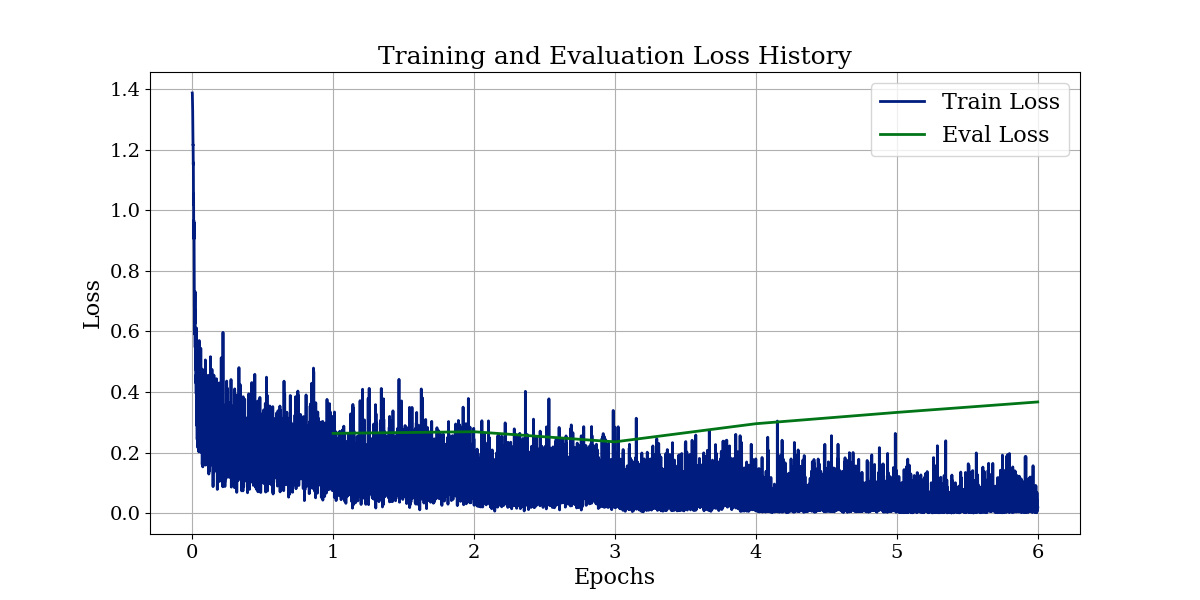
\includegraphics[width=0.7\linewidth]{reports/assignment3/plots/distilbert_training_history.png}
    \caption{Training Curve}
    \label{fig:loss_curve}
\end{figure}

The model achieved an accuracy of 0.9226 on the development set and 0.9424 on the holdout set. The F1-score on the development set was 0.9224 with 0.9424 on the holdout set. A confusion matrix can be seen in Table \ref{tab:confmatrix} below.

\begin{table}[h]
    \centering
    \begin{tabular}{|l|cccc|cccc|}
    \hline
          & \multicolumn{4}{c|}{\textbf{Development Set}} & \multicolumn{4}{c|}{\textbf{Test Set}} \\ \hline
        \textbf{Pred \textbackslash{} Act} & \textbf{World} & \textbf{Sports} & \textbf{Business} & \textbf{Sci/Tech} & \textbf{World} & \textbf{Sports} & \textbf{Business} & \textbf{Sci/Tech} \\ \hline
        \textbf{World}    & 2770 & 45   & 90   & 71   & 1785 & 14   & 57   & 44   \\
        \textbf{Sports}   & 50   & 2731 & 3    & 5    & 10   & 1880 & 6    & 4    \\
        \textbf{Business} & 127  & 13   & 2650 & 249  & 32   & 8    & 1724 & 136  \\
        \textbf{Sci/Tech} & 47   & 25   & 204  & 2920 & 26   & 8    & 93   & 1773 \\ \hline
    \end{tabular}
    \caption{DistilBERT Confusion Matrices}
    \label{tab:confmatrix}
\end{table}

Analysing the table, we can observe that the model has most trouble differentiating Business from the Sci/Tech class in both sets. Interestingly, there is a large difference in performance when the model is predicting Business for World classes on the Development set compared to the test set.

\subsubsection{Robustness}
\paragraph{Length Buckets:} The accuracy and F1 scores were computed for each Bucket. The results can be seen in Table \ref{tab:length_buckets_counts} below, additionally a confusion matrix can be seen for each bucket in Appendix \ref{ap:buckets}. The first thing we need to take into account is the lack of samples in the last 3 bins; a very large majority of samples are between 0-100 tokens, thus in the bins with much larger documents, there are not enough samples to thoroughly evaluate. Thus, we ignore the 200+ length bins. Focusing on these first 4 bins, we observe that the model performs worst for the bin with the shortest sequences in both sets. The metrics increase, and we observe the highest F1 score in the 150-200 bin. On the development set, there is a subtle difference between the F1 score and accuracy on the 150-200 bin. We expect this to be an effect of class imbalance, as can be seen in the confusion matrices in the appendix.
\begin{table}[h]
\centering
\begin{tabular}{|c|c|cc|c|cc|}
\hline
\textbf{Length} & \textbf{\# Dev} & \multicolumn{2}{c|}{\textbf{Dev Set}} & \textbf{\# Test} & \multicolumn{2}{c|}{\textbf{Test Set}} \\ \hline
 &  & Acc & F1 &  & Acc & F1 \\ \hline
0--50   & 5452 & 0.9118 & 0.9110 & 3806 & 0.9364 & 0.9362 \\
50--100 & 6140 & 0.9305 & 0.9301 & 3612 & 0.9477 & 0.9477 \\
100--150& 335  & 0.9582 & 0.9583 & 148  & 0.9595 & 0.9596 \\
150--200& 59   & 0.9492 & 0.9584 & 26   & 0.9615 & 0.9615 \\
200--250& 9    & 0.8889 & 0.8889 & 6    & 1.0000 & 1.0000 \\
250--300& 5    & 1.0000 & 1.0000 & 2    & 1.0000 & 1.0000 \\ \hline
\end{tabular}
\caption{DistilBERT Performance across Input Length Buckets of Different Sample Counts}
\label{tab:length_buckets_counts}
\end{table}

In conclusion, we observe that the model has satisfactory performance across each bucket, with the model performing better for longer sequences (i.e. when more information is present).

\paragraph{Keyword Masking:} After masking out the keywords from Appendix \ref{ap:keywords}, the model is evaluated again. An accuracy of 0.9213 is found on the development set and 0.9399 on the test set. As for the F1-Score, 0.9209 is found on the development set and 0.9397 on the test set. In both cases, there is a very subtle decrease, indicating that something has changed, but the decrease is very subtle; thus, we conclude that the model is not reliant on these particular keywords and is capable of extracting the information from context and not the presence of specific terms. The confusion matrix can be found in Table \ref{tab:keyword_cm}. When comparing this confusion matrix to the one without keyword masking, a few oddities can be observed. Firstly, the performance in sports and business worsened significantly; this seems to have been counteracted by an increase in correctly classified samples in the World and Science/Technology categories. We expect the reason for this might be related to a poor choice of keywords. 

\begin{table}[h]
\centering
\begin{tabular}{|l|cccc|cccc|}
\hline
 & \multicolumn{4}{c|}{\textbf{Dev Set}} & \multicolumn{4}{c|}{\textbf{Test Set}} \\ \hline
\textbf{Pred \textbackslash{} Act} 
& World & Sports & Business & Sci/Tech 
& World & Sports & Business & Sci/Tech \\ \hline

World    
& 2791 & 52  & 70  & 63  
& 1796 & 14  & 40  & 50 \\

Sports   
& 55   & 2726& 5   & 3   
& 10   & 1880& 6   & 4  \\

Business 
& 161  & 16  & 2573& 289 
& 58   & 10  & 1674& 158\\

Sci/Tech 
& 50   & 27  & 153 & 2966
& 26   & 10  & 71  & 1793\\ \hline

\end{tabular}
\caption{DistilBERT Confusion Matrices under Keyword Masking}
\label{tab:keyword_cm}
\end{table}

\subsection{Comparison}
When comparing the DistilBERT to the other models, the main conclusion that can be reached is that it simply performs far better. Focusing in the first place on the accuracy and F1-score, we observe that DistilBERT outperforms both baseline models for both metrics on the development as well as the holdout set. When comparing the types of errors made by the model, we observe that the SVM baseline has a much more uniform distribution across error types, with Business and Sci/Tech being misclassified the most (Appendix \ref{ap:ass1}). When looking at the LSTM, we observe a large decrease in all error types. However, the Business and Sci/Tech confusion decreases the least, with Sci/Tech on Business articles decreasing the least. This trend continues when moving to the DistilBERT model, and a significant decrease is seen in most categories. Nevertheless, the Business and Sci/Tech articles remain by far the hardest for the model to distinguish. 

Although the same additional tests were not conducted for each model, we observe from ablation studies on the LSTM and the length buckets for DistilBERT that both models show improved performance on longer samples. 

\section{Error Analysis}
Looking at the confusion matrix in table \ref{tab:keyword_cm}, we observe that in the test set, the mosoccurringng misclassification happens when the predicted class is Business and the actual class is Sci/Tech. This was also a misclassification that occured regularly in assignment 1 and 2 and can once again be explained by the fact that these two classes have a lot of overlap in vocabulary. In table \ref{tab:misclassifications}, the 10 cases with the lowest confidence error can be found. In reference 1, we can see a quote about Aeolus. The text has no mention of any scientific terms or any technological terms, which leads to misclassification. Reference 2 mentions the company Ford which is doing a recall action. This is something that may be seen in Business articles rather than Sci/Tech articles, which causes a misclassification. The error in reference 3 stems from the same issue as references 1 and 2, there are no terms which lead us to believe that this is Sci/Tech article and it is thus instead classified as a World article. Reference 4 and 5 are Business articles which are classified as World articles. Reference 4 has no Business related vocabulary whatsoever, so it is not surprising that this article is misclassified. Article 5 however does mention money, but also a lawsuit. It is very likely that the misclassification happens because articles that mention lawsuits are usually World articles. Reference 6 does not contain any specific terms that make it a Sci/Tech article, but also does not have any Business terms. It seems logical that this article is misclassified but it is a mystery why it is misclassified as a Business article and not for example a World article, since it does mention Congress. The way of sentencing in article 7, which talks about "Theme park to Open" and "driving force for growth in the city's tourism industry", causes the misclassification as Business class instead of World class. The same error occurs for reference 8, which has sentences like "Bush plans major changes" and "nominating the first female defense secretary". Reference 9 does talk about "Innovative technologies", but also mentions different countries and their presidents, which apparantly has more weight and thus causes a misclassification as World instead of Sci/Tech. For reference 10 the only part of the article that could make it identifiable as a Business article is "the no-strike clause", the rest of the article however talks about a bill being passed which fits more into the World category. 


\section{Discussion}
% What worked what didn't I will write a bit on the tests we did now but this needs to be expanded after Error Analysis 
The DistilBERT model performed significantly better than baseline models. Taking into account improvements to the methodology, a few points come to mind. Firstly, concerning the bins of the Length Bucket evaluation. Considering the large imbalance between buckets, it might have been better to uniformly fill buckets based on a fixed bucket size rather than a fixed-length bucket. This way, the comparison between various bins would have been fairer. This would also answer questions about the behaviour of the model within these large 3000+ sample bins, which is currently not known. Secondly, the keyword masking keywords were not chosen based on a concrete metric. The keywords were manually selected based on perceived presence and correlation with the classes. A more informed selection based on actual within-class frequency of certain words, combined with a cosine similarity threshold to select similar words (currently only the exact words are masked), would have resulted in a more quantifiable comparison, which also would have provided a better test of the model's performance. Additionally, when considering the 50 masked words in the context of a vocabulary consisting of many thousands of words, this might simply be too few words to have a significant effect on performance. 
% Should probably mention the weird training again here. 

% include some error analysis stuff

\section{Limitations}

The Transformer architecture of BERT suffers from inherent scaling limitations. Primarily, the self-attention mechanism possesses a computational complexity of $O(N^2)$ \cite{vaswani2023attentionneed}, which limits the context window. In this project, sequences were truncated to 256 tokens to maintain computational efficiency. While DistilBERT is approximately 40\% smaller and 60\% faster than BERT-base \cite{sanh2020distilbertdistilledversionbert}, this distillation process reduces the model's semantic capacity, potentially leading to the loss of nuanced linguistic details captured by the larger teacher model. Implementing a sliding window approach could allow the model to process longer news articles in chunks, maintaining semantic connections across the entire text without exceeding memory limits.

From error analysis, there is significant confusion between the Business and Sci/Tech categories, which suggests there is an overlap between corporate activities and technological entities in the labelling of the provided dataset; some examples include financial news regarding tech companies being classified as Sci/Tech due to the strong association of the company names with technology, and articles regarding software deals or technology regulations being classified as Business. Using models further pretrained on financial and technological news corpora could help the model distinguish between corporate entities and technical concepts more effectively.

Concerning bias, DistilBERT inherits systematic biases present in the large-scale corpora (Wikipedia and Toronto BookCorpus) used for pre-training, similar to BERT. More severely, the model has been documented to possess significant racial and gender biases in BERT's embeddings and tokenisation. For example, BERT-based models have been shown to encode harmful societal stereotypes, such as associating specific professions with gender \cite{2d985f6031d243c5b17fb284a0e9bb28}. In the context of our dataset and classification task, even if our finetuned AGNews dataset is relatively balanced, the model's underlying understanding of language is grounded in biased associations that can skew predictions in real-world applications. During finetuning on AGNews, an adversarial objective could be added to penalise the model for making predictions based on protected attributes detected in the text.

\newpage
\printbibliography

\suppressfloats[t]
% Here be appendices!
\newpage
\appendix
\addtocontents{toc}{\protect\setcounter{tocdepth}{1}}
\section{GitHub Repository}

The URL to the GitHub Repository: \href{https://github.com/TeunB6/natural-language-processing}{https://github.com/TeunB6/natural-language-processing}. For viewing purposes, the main branch is \texttt{main}.

\section{Model Card}
\label{ap:model_card}

The model card originates from the GitHub repository, and was converted from Markdown-to-PDF using APITemplate.io: \href{https://apitemplate.io/pdf-tools/convert-markdown-to-pdf/}{https://apitemplate.io/pdf-tools/convert-markdown-to-pdf/}.

% dont really think it needs to be cited nah but its aight


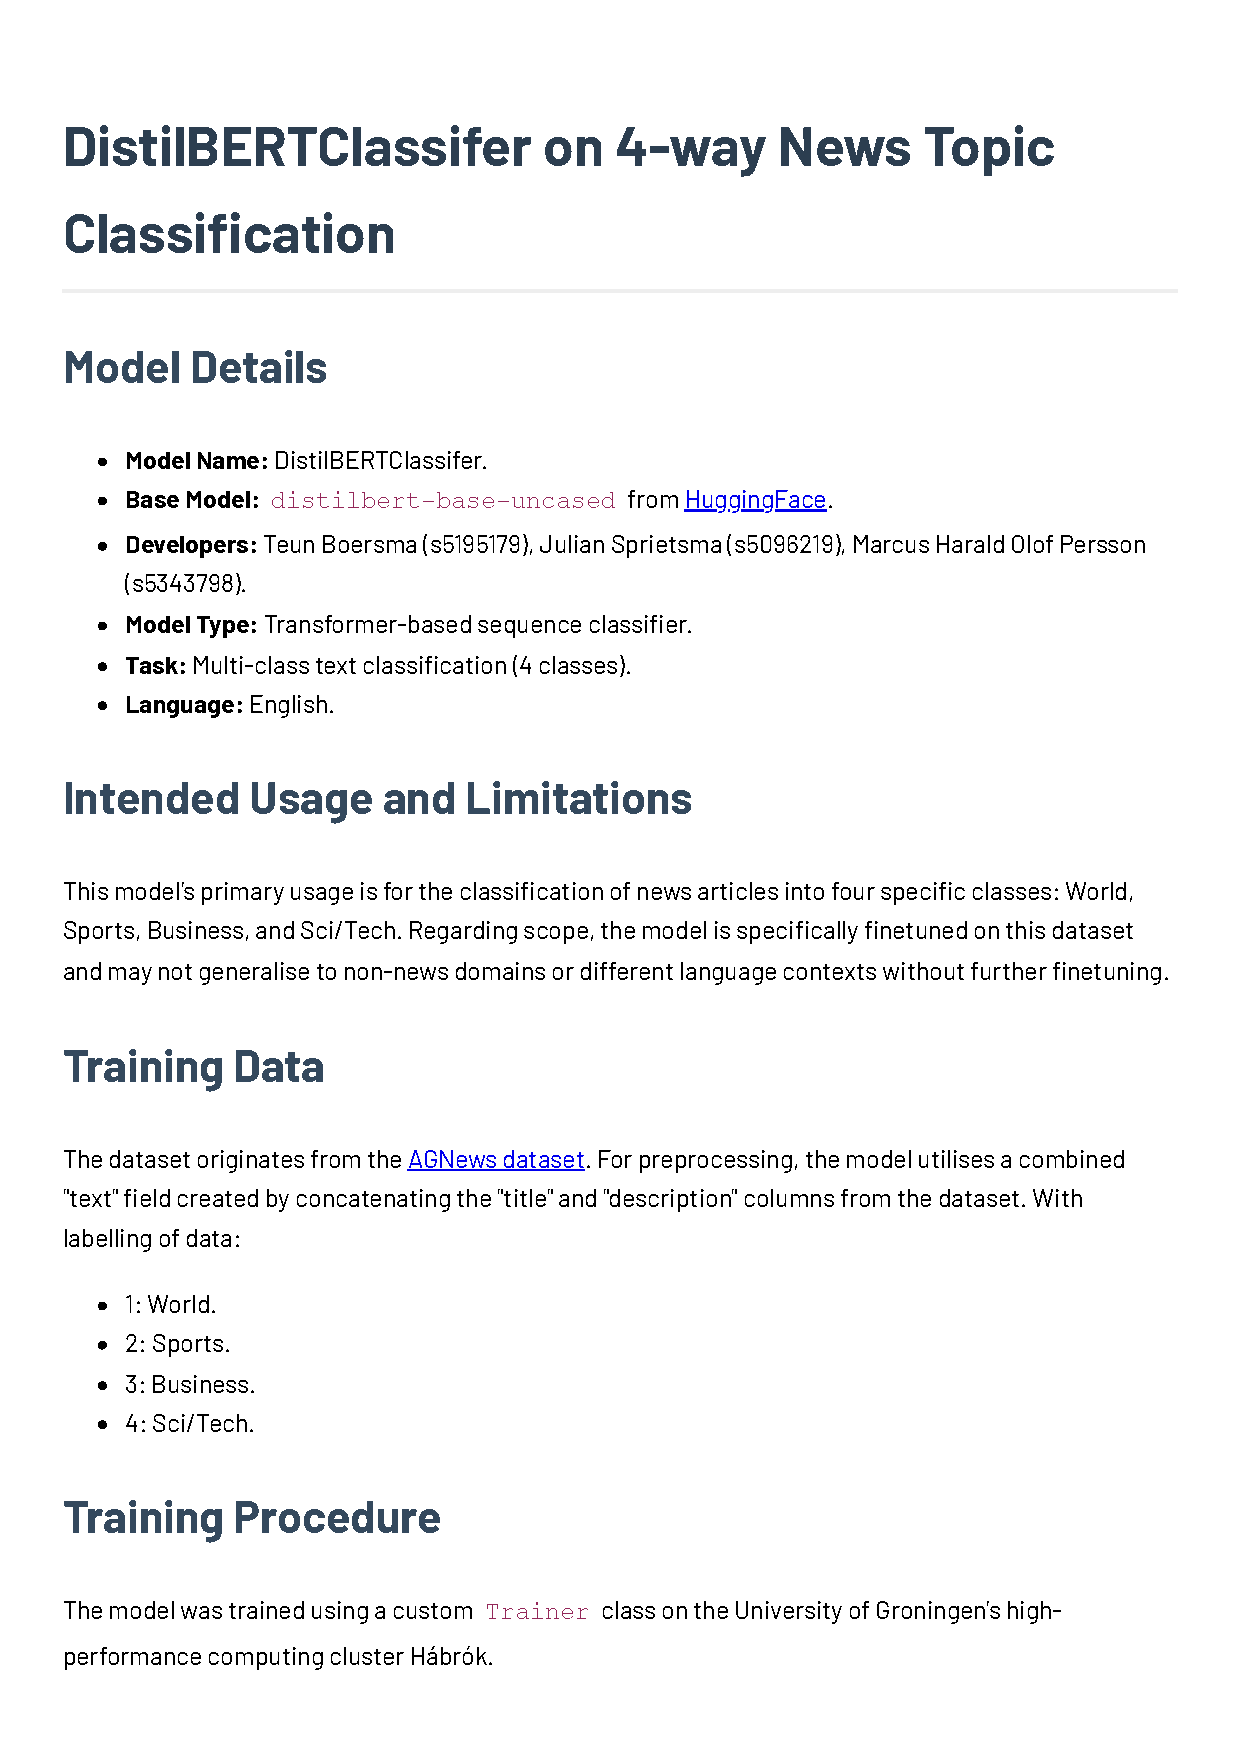
\includepdf[pages=1-, nup=2x2]{reports/assignment3/model_card.pdf} 

\section{AI-Use Statement}
Generative AI was utilised with the purpose and intention of accelerating the development of the project with regard to providing examples on implementing certain features, for example, the CLI UX. Permitted tools were OpenAI ChatGPT, Google Gemini, and GitHub Copilot, with the agreement that training of the models was disabled. Generated code was only used as a reference for comparison to the original written code, to provide any insight on technical scope and considerations we may have missed during development. Autocomplete features were used with human review, and the final product of the project is 100\% human reviewed.

\section{Confusion Matrices per Length Bucket}
\label{ap:buckets}
% added * to sub to avoid it cluttering the table of contents
\subsection{Length Bucket 0--50}
\begin{tabular}{|l|cccc|cccc|}
\hline
 & \multicolumn{4}{c|}{Dev Set} & \multicolumn{4}{c|}{Test Set} \\ \hline
\textbf{Pred \textbackslash{} Act} & World & Sports & Business & Sci/Tech & World & Sports & Business & Sci/Tech \\ \hline
World    & 1139 & 31  & 39  & 45  & 874 & 8   & 25  & 29 \\
Sports   & 23   & 1354& 2   & 1   & 5   & 1005& 3   & 2  \\
Business & 78   & 10  & 987 & 142 & 25  & 4   & 755 & 89 \\
Sci/Tech & 22   & 13  & 75  & 1491& 14  & 6   & 32  & 930\\ \hline
\end{tabular}

\subsection{Length Bucket 50--100}
\begin{tabular}{|l|cccc|cccc|}
\hline
 & \multicolumn{4}{c|}{Dev Set} & \multicolumn{4}{c|}{Test Set} \\ \hline
\textbf{Pred \textbackslash{} Act} & World & Sports & Business & Sci/Tech & World & Sports & Business & Sci/Tech \\ \hline
World    & 1601 & 18  & 34  & 17  & 911 & 2   & 21  & 19 \\
Sports   & 25   & 1360& 0   & 2   & 4   & 868 & 3   & 2  \\
Business & 71   & 7   & 1414& 135 & 21  & 5   & 855 & 61 \\
Sci/Tech & 26   & 19  & 73  & 1338& 11  & 3   & 37  & 789\\ \hline
\end{tabular}

\subsection{Length Bucket 100--150}
\begin{tabular}{|l|cccc|cccc|}
\hline
 & \multicolumn{4}{c|}{Dev Set} & \multicolumn{4}{c|}{Test Set} \\ \hline
\textbf{Pred \textbackslash{} Act} & World & Sports & Business & Sci/Tech & World & Sports & Business & Sci/Tech \\ \hline
World    & 48 & 2 & 0 & 0 & 10 & 0 & 0 & 1 \\
Sports   & 0  & 21& 0 & 0 & 0  & 7 & 0 & 0 \\
Business & 3  & 0 & 149 & 6 & 1  & 1 & 68 & 1 \\
Sci/Tech & 1  & 0 & 2   & 103& 0  & 0 & 2  & 57\\ \hline
\end{tabular}

\subsection{Length Bucket 150--200}
\begin{tabular}{|l|cccc|cccc|}
\hline
 & \multicolumn{4}{c|}{Dev Set} & \multicolumn{4}{c|}{Test Set} \\ \hline
\textbf{Pred \textbackslash{} Act} & World & Sports & Business & Sci/Tech & World & Sports & Business & Sci/Tech \\ \hline
World    & 2 & 0 & 0 & 0 & 1 & 0 & 0 & 0 \\
Sports   & 0 & 1 & 0 & 0 & 0 & 12& 1 & 0 \\
Business & 0 & 0 & 31& 0 & 0 & 0 & 12& 0 \\
Sci/Tech & 3 & 0 & 0 & 22& 0 & 0 & 0 & 0 \\ \hline
\end{tabular}

\subsection{Length Bucket 200--250}
\begin{tabular}{|l|cccc|cccc|}
\hline
 & \multicolumn{4}{c|}{Dev Set} & \multicolumn{4}{c|}{Test Set} \\ \hline
\textbf{Pred \textbackslash{} Act} & World & Sports & Business & Sci/Tech & World & Sports & Business & Sci/Tech \\ \hline
World    & 4 & 1 & 0 & 0 & 1 & 0 & 0 & 0 \\
Sports   & 0 & 4 & 0 & 0 & 0 & 5 & 0 & 0 \\
Business & 0 & 0 & 0 & 0 & 0 & 0 & 0 & 0 \\
Sci/Tech & 0 & 0 & 0 & 0 & 0 & 0 & 0 & 0 \\ \hline
\end{tabular}

\subsection{Length Bucket 250--300}
\begin{tabular}{|l|cccc|cccc|}
\hline
 & \multicolumn{4}{c|}{Dev Set} & \multicolumn{4}{c|}{Test Set} \\ \hline
\textbf{Pred \textbackslash{} Act} & World & Sports & Business & Sci/Tech & World & Sports & Business & Sci/Tech \\ \hline
World    & 1 & 0 & 0 & 0 & 2 & 0 & 0 & 0 \\
Sports   & 0 & 4 & 0 & 0 & 0 & 0 & 0 & 0 \\
Business & 0 & 0 & 0 & 0 & 0 & 0 & 0 & 0 \\
Sci/Tech & 0 & 0 & 0 & 0 & 0 & 0 & 0 & 0 \\ \hline
\end{tabular}

\section{Masked Keywords}
\label{ap:keywords}
The keywords were selected based on their appearance within the documents. For Business, many different terms related to financial markets are included. Science and Technology articles often reference specific fields that were included in the list, as well as people with titles such as scientist or professor. For sports, a few specific sports were highlighted as well as some common themes as the olympics, score and tournament. Lastly, world news in the dataset mostly consists of conflicts and wars. As keywords, a few commonly occurring countries as well as related terms like conflict, battle and treaty often occurred in these articles. 

\begin{table}[h]
\centering
\begin{tabular}{llll}
\textbf{Business} & \textbf{Science/Tech} & \textbf{Sports} & \textbf{World} \\ \hline

finance & psychology & football & conflict \\
economy & physics & basketball & battle \\
investment & chemistry & tennis & treaty \\
market & scientist & athlete & climate \\
stocks & professor & coach & terrorism \\
banking & biology & tournament & refugee \\
entrepreneur & ecology & league & iran \\
startup & molecular & championship & israel \\
corporate & quantum & olympics & war \\
trade & astronomy & score & syria \\

\end{tabular}
\caption{Keyword categories used for masking}
\end{table}

\section{Cases of misclassification}
\begin{table}[H]
\begin{longtable}{| m{2em} | m{25em} | m{5em} | m{5em} |}
        \hline
        \textbf{Ref} & \textbf{Text} & \textbf{Actual} & \textbf{Predicted} \\ \hline
        1 & The Bag of Aeolus quot;Aeolus was keeper of the winds. He gave a bag of evil winds to Odysseus, instructing him to keep it closed while a good breeze wafted him home. & Sci/Tech & World \\ \hline
        
        2 & Ford to Recall 474,000 SUVs Worldwide (Reuters) Reuters - Ford Motor Co said on Friday it\was recalling about 474,000 Escape and Mazda Tribute sport\utility vehicles globally because the accelerator cable may\prevent the engine from returning to the idle position, which\could increase stopping distance and result in a crash. & Sci/Tech & Business \\ \hline
        
        3 & Will there be peace in Great Lakes region? To coordinate and cooperate or not to, that is where the rub is, and that is the key issue when it comes to answering the question whether there will be peace in the Great Lakes region. & Sci/Tech & World \\ \hline
        
        4 & Future Doctors, Crossing Borders Students at the Mount Sinai School of Medicine learn that diet and culture shape health in East Harlem. & Business & World \\ \hline
        
        5 & Panel Urges N.Y. to Pay \$14 Billion More for City Schools Court-appointed referees recommended the state pay an additional \$14 billion over four years to improve New York City schools. & Business & World \\ \hline
        
        6 & A wandering Congress trips over the US Constitution That is the one-word message of advice that citizens wanted to send to members of Congress at the end of last week. Both the House of Representatives and the Senate looked as if they are having trouble seizing & Sci/Tech & Business \\ \hline
        
        7 & HK Disneyland Theme Park to Open in September Hong Kong's Disneyland theme park will open on Sept. 12, 2005 and become the driving force for growth in the city's tourism industry, Hong Kong's government and Walt Disney Co. & World & Business \\ \hline
        
        8 & Staying or Going? Some Possibilities if Bush Wins President Bush plans major changes in his Cabinet if he wins a second term -- perhaps nominating the first female defense secretary and first black -- but very little change among the small group of his closest advisors. & World & Business \\ \hline

        9 & India, Russia must work together on new tech: Putin BANGALORE, DEC 5: Russian President Vladimir Putin has called upon India and Russia to work together on innovative technologies with younger generation taking the lead. & Sci/Tech & World \\ \hline
        
        10 & Changes to Nigeria union bill The Nigerian senate passes a bill to curb the power of the trade unions, but amends the no-strike clause. & Business & World \\ \hline

\caption{The 10 lowest confidence errors}
\label{tab:misclassifications}
\end{longtable}
\end{table}


\section{Assignment 1}
\label{ap:ass1}

\includepdf[pages=1-, nup=2x2]{reports/assignment3/old_assignments/assignment_1.pdf} 
\section{Assignment 2}
\label{ap:ass2}

\includepdf[pages=1-, nup=2x2]{reports/assignment3/old_assignments/assignment_2.pdf} 

\newpage
\end{document}